\clearpage
\section*{\currfilename}

\pgfdeclarelayer{background}
\pgfdeclarelayer{foreground}
\pgfsetlayers{background,main,foreground}
% Define a few styles and constants
\tikzstyle{sensor}=[draw, fill=blue!20, text width=5em, text centered, minimum height=2.5em]
\tikzstyle{ann} = [above, text width=5em]
\tikzstyle{naveqs} = [sensor, text width=6em, fill=red!20, minimum height=12em, rounded corners]
\def\blockdist{5}
\def\edgedist{2.5}

\begin{tikzpicture}
  \node (block3) [squareblock, label=below:{\shortstack[c]{\bf Nonlinear Equations\\ \bf of Motion}}, minimum width=6cm, inner sep=0mm] {\centering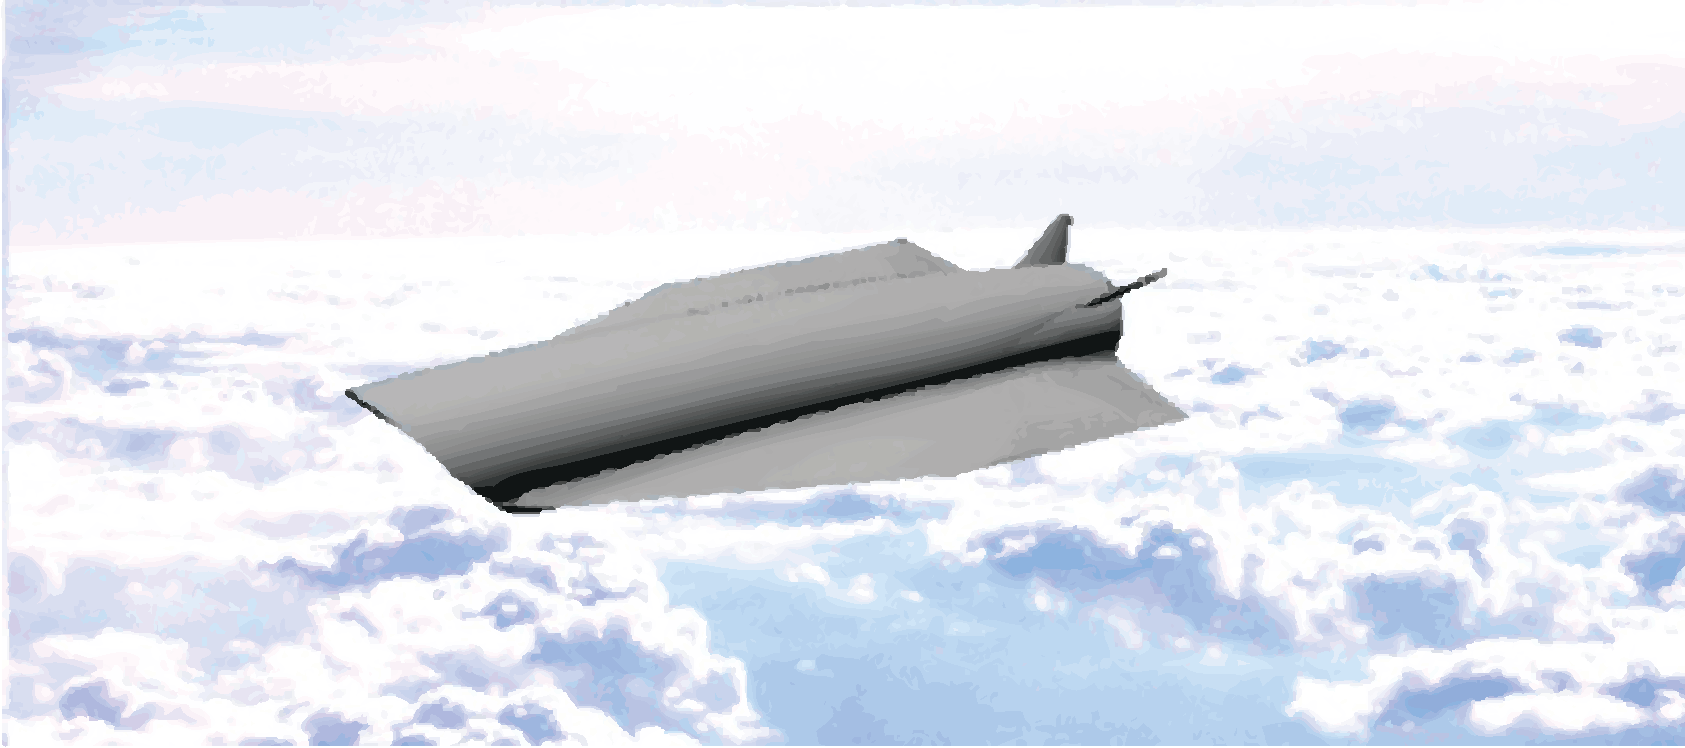
\includegraphics[width=6cm]{../fig/ghvclouds.pdf}};
  \node (summer) [whitesum, left of=block3, node distance=4cm] {};
  \path (naveq.145)+(-\blockdist,0) node (block1) [squareblock, minimum width=2.5cm] {Baseline};
  \draw[->](block1) -| node[right, pos=0.8]{$+$} (summer);
  \draw[->](summer) -- node[above,pos=0.5]{$u$} (block3);
  \draw[->](block3) -- (block4);
\end{tikzpicture}
